\documentclass{article}
\usepackage{neurips_2026}
\usepackage[utf8]{inputenc}
\usepackage[T1]{fontenc}
\usepackage{hyperref}
\usepackage{url}
\usepackage{booktabs}
\usepackage{amsfonts,amsmath,amssymb,amsthm}
\usepackage{nicefrac}
\usepackage{microtype}
\usepackage{xcolor}
\usepackage{graphicx}
\usepackage{enumitem}
\newtheorem{proposition}{Proposition}

\title{How Many Benchmarks Must You Run? Choosing a Few and Inferring the Rest from Leaderboard Score Matrices}

\author{Anonymous Author(s)}

\begin{document}
\maketitle

\begin{abstract}
A new model is usually evaluated on many benchmarks, each costing compute and time, yet public leaderboards show that benchmark scores are strongly related. We ask: with a budget of $k$ benchmarks out of $N$, which should be run, how well can the other scores be inferred from a history of models with missing cells, and how large must $k$ be?
We propose a Gaussian-conditional predictor fitted to pairwise-complete covariances and a greedy variance-reduction rule that chooses the benchmarks, and give theory: a closed-form error with an irreducible per-benchmark floor, a sandwich $k=\Theta(r/\epsilon)$ for random selection under a rank-$r$ factor model, a spectral lower bound for any selection, and the $k/(M-k-1)$ price of unstructured regression; simulations confirm each.
On seven public matrices (MTEB subsets, Open LLM Leaderboard, HELM Lite, LiveBench) we hold out whole models and a fixed set of target benchmarks, so that all selectors are scored on identical targets, with bootstrap CIs.
On MTEB (189 models $\times$ 280 tasks), one well-chosen task gives $R^2=0.52$ against the mean baseline (random: 0.39), five give 0.71 and ten 0.76; accuracy saturates near 0.80 for every selector, leaving $\sim$7 points of RMSE on single tasks but $\sim$1 point on the average of the remaining scores.
Selection reduces MSE by 21\% at $k=1$ and 13\% at $k=10$ versus random and not detectably at $k=40$; running the most commonly evaluated benchmarks is worse than random. The benefit survives new organisations and later releases at small $k$, shrinks with sparse or small histories, and vanishes in homogeneous pools and on the smallest LLM matrices. Scoring selectors on the benchmarks left over after selection inflates their advantage.
\end{abstract}

\section{Introduction}
\label{sec:intro}

Evaluating a model means running it on many benchmarks, and every benchmark costs compute, time and people. Public leaderboards have meanwhile accumulated large model$\times$benchmark score matrices, and the scores of different benchmarks are far from independent. This suggests a concrete budgeted problem. Given a history of $M$ models scored on $N$ benchmarks (with missing cells), a new model can only be run on $k\ll N$ benchmarks: \emph{which $k$, and how accurately can the remaining $N-k$ scores be inferred? How large must $k$ be?}

Existing efficiency work mostly reduces the number of \emph{items inside a benchmark} \citep{vivek2024anchor,polo2024tiny,kipnis2024metabench,perlitz2024efficient}, and work on relations between benchmarks mostly asks \emph{whether} they agree or lie on a low-dimensional manifold \citep{perlitz2024benchbench,ruan2024observational,polo2024sloth}. We study the missing middle: the \emph{choice of whole benchmarks} to run for a new model, with evaluation designed so that the answer is unbiased and comes with uncertainty. We make four contributions.
\begin{enumerate}[leftmargin=1.5em,itemsep=1pt,topsep=1pt]
\item \textbf{A method} (\S\ref{sec:method}): a Gaussian conditional predictor fitted to pairwise-complete covariances of the history, with a greedy variance-reduction rule for choosing $S$ that costs $O(N^2k)$, together with six alternative predictors (mean, averaging, factor model, SVD imputation, nearest neighbours, a blend) and seven alternative selection rules (including random).
\item \textbf{Theory} (\S\ref{sec:theory}, Appendix~\ref{app:proofs}): a closed-form error with an irreducible per-benchmark floor (adaptive selection gains nothing under the Gaussian model); a sandwich $\sum_i g_i/(1+kg_i)\le\text{excess}\le r/(k-r-1)$ for random selection, hence $k=\Theta(r/\epsilon)$; a spectral lower bound valid for \emph{any} selection; and the $k/(M-k-1)$ price of unstructured regression on a finite history. All are verified numerically.
\item \textbf{Evidence on seven real matrices} (three nested subsets of MTEB, Open LLM Leaderboard, two HELM Lite versions, LiveBench), under random-model, new-organisation and temporal splits, with bootstrap CIs, and ablations of history size, missingness, benchmark pool and score transform.
\item \textbf{A protocol point}: scoring each selector on the benchmarks \emph{left over} after its own selection inflates the apparent advantage of informative selection; we score all methods on identical held-out targets.
\end{enumerate}

\paragraph{Findings in brief.} On MTEB-main, one well-chosen task gives $R^2=0.52$ (random: 0.39), five give 0.71, ten 0.76, and accuracy then saturates near 0.80 for \emph{all} selectors. Selection matters mostly for $k\le10$ (MSE $-21\%$ at $k=1$, nil at $k=40$), the most commonly evaluated benchmarks are \emph{worse} than random ones, the benefit shrinks with sparse or small histories, in homogeneous pools and on the smallest LLM matrices, and the fitted Gaussian predicts its own held-out error to within $\sim$10\%, which lets the budget be planned from the history.

\section{Related work}
\label{sec:related}

\paragraph{Cheaper evaluation within one benchmark.}
Most work on evaluation cost shrinks a \emph{single} benchmark: choosing few items that preserve model rankings or scores, via clustering of model confidences \citep{vivek2024anchor}, item-response models \citep{polo2024tiny}, or a sparse, psychometrically selected item set built from thousands of models' results on six benchmarks \citep{kipnis2024metabench}; \citet{perlitz2024efficient} frame the general problem of ``efficient benchmarking'' and study how far a benchmark can be reduced. Our question is orthogonal: which \emph{whole benchmarks} to run, and what they say about the others.

\paragraph{Relations between benchmarks.}
Large suites report many tasks per model \citep{hendrycks2020mmlu,muennighoff2022mteb,liang2022helm,zhuo2024bigcodebench}, and judge-based or arena-style evaluations add further axes \citep{zheng2023judging}. Whether benchmarks agree is itself sensitive to methodological choices \citep{perlitz2024benchbench}. Observational scaling laws \citep{ruan2024observational} and Sloth \citep{polo2024sloth} exploit the low-dimensional structure of public benchmark scores to predict performance on some benchmarks from others, often as a function of model scale or family. We use no scale or family information, treat the choice of the observed benchmarks as the object of study, and ask how accurate the inference is as a function of the number of benchmarks and of \emph{which} ones.

\paragraph{Subset selection and cold-start elicitation.}
Choosing $k$ variables to predict the rest is sensor placement in a Gaussian process \citep{krause2008near}, linear subset selection \citep{das2011submodular}, and column-subset selection. Eliciting a few ratings from a new user is the cold-start problem of recommender systems, studied extensively with active learning \citep{elahi2016survey}, and computerized adaptive testing does the same for test-takers. Leaderboards differ in ways that matter: the matrix is small and dominated by one general factor, cells are missing in a model-dependent way, and the new row may be systematically better than the history. We port the Gaussian machinery, state what it implies for $k$, and test it under these conditions. The predictor side is matrix completion \citep{mazumder2010softimpute} and probabilistic PCA/factor analysis \citep{tipping1999ppca}; covariance estimation uses shrinkage \citep{ledoit2004well}.

\section{Problem setting and method}
\label{sec:method}

\paragraph{Setting.}
A history matrix $X\in(\mathbb{R}\cup\{\text{NA}\})^{M\times N}$ holds the scores of $M$ models on $N$ benchmarks, with missing cells.
A new model arrives. The evaluator may run any $k$ benchmarks $S\subset[N]$ (the \emph{budget}) and must then predict the model's scores on benchmarks it will not run.
We standardize every benchmark with its training mean and standard deviation, so that a model's score vector is $z\in\mathbb{R}^N$, and measure error by the \emph{standardized MSE} on the targets (also reported in score points).
Two decisions are to be made: \emph{which} $S$ to run (selection), and \emph{how} to infer $z_{T}$ from $z_S$ (prediction).
Both may use only $X$.

\paragraph{Predictors.}
Our main predictor treats $z\sim\mathcal N(\mu,\Sigma)$ and predicts with the Gaussian conditional mean $\hat z_T=\mu_T+\Sigma_{TS}\Sigma_{SS}^{-1}(z_S-\mu_S)$, which is Bayes-optimal under squared loss if the model holds.
We estimate $\Sigma$ from \emph{pairwise-complete} observations of $X$ (so missing cells are handled without imputation), project it to the PSD cone, and shrink it toward the identity on the correlation scale, $\Sigma_\kappa=(1-\kappa)\hat C+\kappa I$, with $\kappa$ chosen on a validation split of the \emph{training} models (\textsc{Gauss}).
We compare against: the benchmark mean (\textsc{Mean}); the \emph{average of the benchmarks run}, rescaled per target (\textsc{AvgShift}); a rank-$r$ probabilistic factor model $z=\mu+\Lambda f+\varepsilon$, $\varepsilon_j\sim\mathcal N(0,\psi_j)$, fitted by EM with missing data \citep{tipping1999ppca} and folded in by the posterior of $f$ (\textsc{FA}); iterative-SVD imputation with ridge fold-in in the spirit of soft-impute \citep{mazumder2010softimpute} (\textsc{ISVD}); $K$-nearest models (\textsc{kNN}); and a blend of pairwise and factor-model covariance (\textsc{Hybrid}). All hyper-parameters (rank, shrinkage, $K$) are tuned by an inner split of the training rows.

\paragraph{Selection rules.}
For a Gaussian model the expected squared error on benchmark $j$ after observing $S$ is $v_j(S)=\Sigma_{jj}-\Sigma_{jS}\Sigma_{SS}^{-1}\Sigma_{Sj}=\mathrm{Var}(z_j\mid z_S)$ and does not depend on the observed values.
We choose $S$ to minimize the pool-level objective $F(S)=\sum_{j}v_j(S)$ (members of $S$ contribute zero), greedily:
\begin{equation}
 j_{t+1}\in\arg\max_{j\notin S_t}\ \frac{\sum_{i}\mathrm{Cov}(z_i,z_j\mid z_{S_t})^2}{\mathrm{Var}(z_j\mid z_{S_t})}
 \label{eq:greedy}
\end{equation}
(\textsc{Greedy}; a rank-one downdate of the residual covariance per step, $O(N^2k)$ in total, a few milliseconds for $N\approx 300$).
Baselines: \textsc{Random}; \textsc{Most-evaluated} (the benchmarks that most models report---what a practitioner would run by default); \textsc{Most-correlated} (largest mean absolute correlation with the others, which ignores redundancy); \textsc{$k$-medoids} on $1-|\rho|$; \textsc{Greedy-MaxVar} (largest conditional variance, the entropy rule of \citet{krause2008near}); \textsc{Greedy-MI} (the mutual-information rule of \citet{krause2008near}); and top factor-model SNR. Selection is always restricted to the benchmarks the new model has actually been run on (the \emph{pool}), and uses only training rows.

\subsection{Theory: what limits accuracy, and how large $k$ must be}
\label{sec:theory}
All statements are for the Gaussian model; proofs are in Appendix~\ref{app:proofs}, and each is checked numerically in \S\ref{sec:exp_theory}.

\begin{proposition}[Closed form, floor, no gain from adaptivity]\label{prop:closed}
If $\Sigma=\Lambda\Lambda^\top+\Psi$ with $\Lambda\in\mathbb{R}^{N\times r}$, then
$v_j(S)=\psi_j+\lambda_j^\top\big(I+\Lambda_S^\top\Psi_S^{-1}\Lambda_S\big)^{-1}\lambda_j .$
Hence $v_j(S)\ge\psi_j$ for every $S$ (an irreducible per-benchmark floor), $v_j$ is non-increasing in $S$, and $v_j(S)$ does not depend on the observed scores: choosing benchmarks sequentially, after seeing results, cannot beat choosing the same number in advance.
\end{proposition}

\begin{proposition}[Random selection: $k$ must scale with the rank]\label{prop:random}
Let the loading rows be i.i.d.\ $\mathcal N(0,\sigma^2G)$, $\Psi=\sigma^2I$, with eigenvalues $g_1\ge\dots\ge g_r$ of $G$, and let $S$ be a uniformly random set of $k$ benchmarks, $j\notin S$. Then
\[
 \sum_{i=1}^r\frac{g_i}{1+k g_i}\ \le\ \frac{\mathbb{E}\,v_j(S)}{\sigma^2}-1\ \le\ \frac{r}{k-r-1}\qquad(k\ge r+2).
\]
For equal $g_i=g$, the excess error over the floor is therefore $\le\epsilon\sigma^2$ only if $k\ge r/\epsilon-1/g$, and is guaranteed once $k\ge r(1+1/\epsilon)+1$: $k=\Theta(r/\epsilon)$. A factor with small strength $g_i$ is not recovered until $k\gtrsim 1/g_i$.
\end{proposition}

\begin{proposition}[No selection beats the spectrum]\label{prop:tail}
For any Gaussian $\Sigma$ and \emph{any} $S$ with $|S|=k$, $F(S)\ge\sum_{i>k}\lambda_i(\Sigma)$. Under the factor model with $\Psi=\sigma^2 I$ and $k\ge r$ this is $\sigma^2(N-k)$, i.e.\ $\ge\sigma^2$ per target.
\end{proposition}

\begin{proposition}[Finite history: unstructured regression pays $k/(M-k-1)$]\label{prop:ols}
Under Gaussian design with known means, regressing each target on the $k$ selected benchmarks by least squares on $M>k+1$ complete training rows has $\mathbb{E}[\text{test MSE}]=v_j(S)\,(1+k/(M-k-1))$.
\end{proposition}

\paragraph{Greedy quality.} $f(S)=\mathrm{tr}\,\Sigma-F(S)=\sum_j\mathrm{Var}(z_j)R^2_j(S)$ is a non-negative combination of squared multiple correlations, so by \citet{das2011submodular} its submodularity ratio is at least $\lambda_{\min}$ of the correlation matrix and greedy attains $\ge(1-e^{-\lambda_{\min}})$ of the optimum. This guarantee is weak when benchmarks are strongly collinear (small $\lambda_{\min}$); we therefore measure the greedy/optimal ratio directly (\S\ref{sec:exp_theory}).

\paragraph{Cost and applicability.} Fitting costs one pairwise covariance ($O(MN^2)$) plus tuning; selection is $O(N^2k)$; prediction is one $k\times k$ solve. The history must contain enough co-observations (we require $\ge5$ models per pair, else correlation 0) and the new model is assumed exchangeable with it; \S\ref{sec:exp_shift} tests violations.

\section{Experiments}
\label{sec:exp}

\paragraph{Data.}
All matrices are public and version-pinned (Appendix~\ref{app:repro}). \textbf{MTEB} \citep{muennighoff2022mteb,mtebresults}: one score per (embedding model, task), the task's main metric on its test split (averaged over language subsets; a task enters only with the modal subset signature). From 531 models $\times$ 1,172 tasks (11\% filled) we keep tasks with $\ge100$ models and models with $\ge60$ of those tasks: \textbf{MTEB-main} (189 models $\times$ 280 tasks, 77\% filled, on average 215 observed tasks per model); \textbf{MTEB-dense} ($\ge150$ models/task, $\ge80$ tasks/model: 175 $\times$ 164, 90\%) and \textbf{MTEB-eng} (English tasks only: 185 $\times$ 91). LLM leaderboards are small in $N$: \textbf{OpenLLM-LB} (6 benchmarks $\times$ 4,496 models, complete; \citealp{openllm2024}), \textbf{HELM-Lite-22} (22 scenario/sub-scenario scores $\times$ 91 models; \citealp{helmlite,liang2022helm}), its 10-scenario version, and \textbf{LiveBench-7} (7 task scores $\times$ 158 models with $\ge5$ of them; \citealp{white2024livebench}). In every matrix (Table~\ref{tab:data}) one factor carries 57--74\% of the correlation spectrum, but 90\% of it needs $n_{90}=3$--20 components: a dominant general factor plus a long tail.

\begin{table}[t]
\centering\small
\caption{Matrices. $\lambda_1/N$: top eigenvalue share of the pairwise correlation matrix; PR: participation ratio; $n_{90}$: components for 90\% of the spectrum; $\rho$: off-diagonal correlation.}
\label{tab:data}
\begin{tabular}{lrrrrrrr}\toprule
Dataset & Models & Bench. & Density & $\lambda_1/N$ & PR & $n_{90}$ & mean $\rho$ \\\midrule
MTEB-main & 189 & 280 & 0.77 & 0.57 & 2.9 & 20 & 0.56 \\
MTEB-dense & 175 & 164 & 0.90 & 0.60 & 2.6 & 15 & 0.58 \\
MTEB-eng & 185 & 91 & 0.70 & 0.68 & 2.1 & 10 & 0.65 \\
HELM-Lite-22 & 91 & 22 & 1.00 & 0.58 & 2.8 & 8 & 0.52 \\
HELM-Lite-10 & 91 & 10 & 1.00 & 0.63 & 2.3 & 4 & 0.55 \\
LiveBench-7 & 158 & 7 & 0.89 & 0.73 & 1.8 & 4 & 0.68 \\
OpenLLM-LB & 4496 & 6 & 1.00 & 0.74 & 1.8 & 3 & 0.67 \\
\bottomrule\end{tabular}

\end{table}

\paragraph{Protocol.}
\emph{Rows are held out}, never cells: models are split into 5 folds (3 repeats with different fold seeds for MTEB, 10 for HELM/LiveBench, 1 for OpenLLM), all fitting, tuning and selection use training rows only, and each held-out model is a ``new model'' that reveals $k$ scores. For every held-out model with observed set $C$ we draw a set $T_0$ of \emph{held-out targets} (30\% of $C$; two draws per model; for $N\le12$ every single benchmark in turn) and let each selector choose $S$ from the pool $C\setminus T_0$. \emph{All selectors and predictors are scored on the same $T_0$.} Selection is thus restricted to what the model actually has scores for, and neither $S$ nor the baseline determines the targets (\S\ref{sec:exp_pitfall} shows why this matters). Curves compare the same (model, $T_0$) cells at every $k$. We report the standardized MSE and $R^2=1-\mathrm{MSE}/\mathrm{MSE}_{\textsc{mean}}$, where \textsc{mean} predicts each target by its training mean; random selection averages 10 draws per cell. Uncertainty: 95\% percentile bootstrap over held-out \emph{models}, resampled jointly for paired differences (Wilcoxon $p$-values are in the released tables). Besides random splits we use \emph{new-organisation} splits (5 folds by organisation prefix, MTEB) and a \emph{temporal} split (training on the oldest 70\% of models by release/submission date, testing on the rest: 53 MTEB models, 1,332 OpenLLM models).

\subsection{How accurate is inference from $k$ benchmarks, and does selection matter?}
\label{sec:exp_main}
Figure~\ref{fig:main} and Table~\ref{tab:main} give the central result. On MTEB-main the average held-out model has 215 observed tasks, 30\% of which (about 65) are the held-out targets, and the mean baseline has RMSE 17.4 score points per target. With \emph{one} well-chosen task, $R^2=0.52$ (RMSE 11.0 points); with five, 0.71 (8.0 points); with ten, 0.76 (7.2 points). After that returns diminish quickly: at $k=40$ both greedy and random reach $R^2\approx0.80$ (6.7 vs.\ 6.4 points). The plateau is reached by every selector and by the best predictors (Appendix Table~\ref{tab:pred}): the unexplained 20\% is consistent with benchmark-specific variation that the other benchmarks do not carry (we cannot separate it from evaluation noise). It is far smaller for \emph{aggregates}: the mean of the held-out scores is predicted with mean absolute error 1.7 points at $k=5$ and 1.3 at $k=10$ (random: 2.7 and 1.8; mean baseline: 10.5), because benchmark-specific errors average out (Appendix~\ref{app:more}).

\begin{figure}[t]
\centering
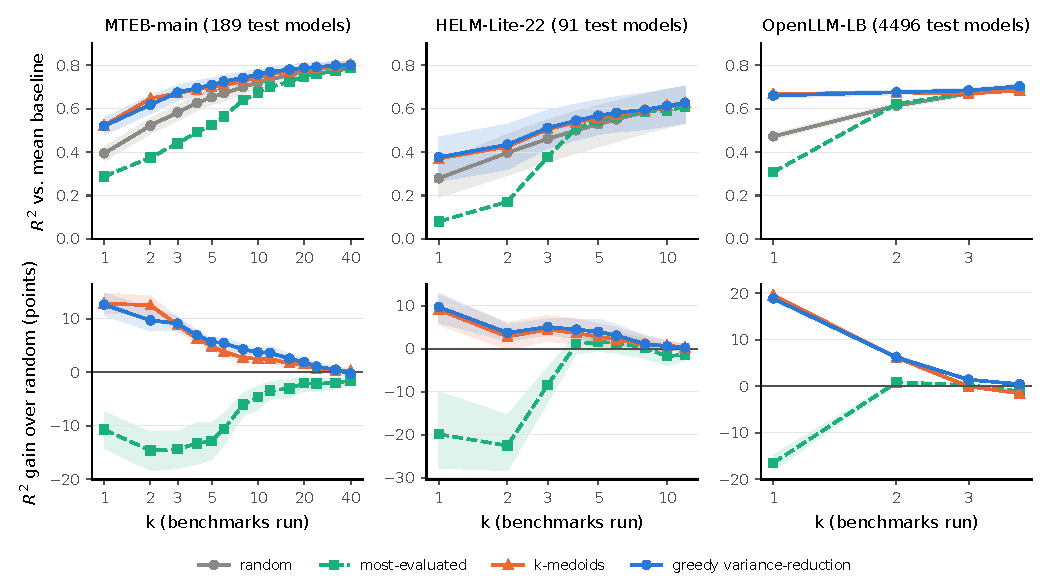
\includegraphics[width=\linewidth]{figs/main_curves.pdf}
\caption{Held-out accuracy vs.\ number of benchmarks run $k$ (Gaussian predictor). Top: $R^2$ vs.\ the mean baseline; bottom: paired $R^2$ gain over random selection; bands: 95\% bootstrap CIs over models. On complete matrices (OpenLLM-LB, HELM) ``most-evaluated'' is column order. Other matrices: Fig.~\ref{fig:app_curves}.}
\label{fig:main}
\end{figure}

\begin{table}[t]
\centering\small
\caption{$R^2$ [95\% CI] at $k$ benchmarks run, Gaussian predictor, random splits of models. Bold: best selector per column (ties at two decimals); ``--'': $k$ not available for this matrix.}
\label{tab:main}
\resizebox{\linewidth}{!}{\begin{tabular}{llcccc}\toprule
Dataset (split) & Selector & $k{=}1$ & $k{=}3$ & $k{=}5$ & $k{=}10$ \\\midrule
MTEB-main (rand) & random & 0.39 \scriptsize[0.36,0.42] & 0.58 \scriptsize[0.54,0.62] & 0.65 \scriptsize[0.62,0.68] & 0.72 \scriptsize[0.69,0.75] \\
 & most-evaluated & 0.29 \scriptsize[0.24,0.33] & 0.44 \scriptsize[0.38,0.48] & 0.52 \scriptsize[0.47,0.57] & 0.67 \scriptsize[0.63,0.71] \\
 & k-medoids & \textbf{0.52} \scriptsize[0.48,0.56] & \textbf{0.67} \scriptsize[0.64,0.71] & 0.70 \scriptsize[0.67,0.73] & 0.75 \scriptsize[0.72,0.77] \\
 & greedy variance-reduction & \textbf{0.52} \scriptsize[0.48,0.56] & \textbf{0.67} \scriptsize[0.64,0.71] & \textbf{0.71} \scriptsize[0.68,0.74] & \textbf{0.76} \scriptsize[0.73,0.78] \\
\midrule
HELM-Lite-22 (rand) & random & 0.28 \scriptsize[0.19,0.35] & 0.46 \scriptsize[0.35,0.55] & 0.53 \scriptsize[0.42,0.62] & \textbf{0.61} \scriptsize[0.51,0.69] \\
 & most-evaluated & 0.08 \scriptsize[0.04,0.12] & 0.38 \scriptsize[0.26,0.46] & 0.54 \scriptsize[0.44,0.63] & 0.59 \scriptsize[0.49,0.68] \\
 & k-medoids & 0.37 \scriptsize[0.26,0.46] & \textbf{0.51} \scriptsize[0.42,0.58] & 0.56 \scriptsize[0.47,0.63] & \textbf{0.61} \scriptsize[0.52,0.69] \\
 & greedy variance-reduction & \textbf{0.38} \scriptsize[0.26,0.47] & \textbf{0.51} \scriptsize[0.42,0.59] & \textbf{0.57} \scriptsize[0.48,0.64] & \textbf{0.61} \scriptsize[0.52,0.69] \\
\midrule
OpenLLM-LB (rand) & random & 0.47 \scriptsize[0.46,0.49] & 0.67 \scriptsize[0.66,0.68] & -- & -- \\
 & most-evaluated & 0.31 \scriptsize[0.29,0.33] & 0.67 \scriptsize[0.66,0.68] & -- & -- \\
 & k-medoids & \textbf{0.67} \scriptsize[0.66,0.68] & 0.67 \scriptsize[0.66,0.68] & -- & -- \\
 & greedy variance-reduction & 0.66 \scriptsize[0.65,0.67] & \textbf{0.68} \scriptsize[0.67,0.69] & -- & -- \\
\midrule
LiveBench-7 (rand) & random & 0.47 \scriptsize[0.40,0.53] & 0.61 \scriptsize[0.54,0.67] & -- & -- \\
 & most-evaluated & 0.50 \scriptsize[0.41,0.58] & \textbf{0.64} \scriptsize[0.58,0.69] & -- & -- \\
 & k-medoids & \textbf{0.53} \scriptsize[0.46,0.60] & 0.60 \scriptsize[0.54,0.66] & -- & -- \\
 & greedy variance-reduction & \textbf{0.53} \scriptsize[0.45,0.59] & 0.59 \scriptsize[0.53,0.65] & -- & -- \\
\bottomrule
\end{tabular}
}
\end{table}

\emph{Selection matters most at the smallest budgets.} On MTEB-main, greedy selection lowers the MSE of random selection by 21\% [17, 25] at $k=1$, 16\% [14, 19] at $k=5$, 13\% [12, 15] at $k=10$, 8\% [6, 11] at $k=20$, and not detectably at $k=40$ ($-1\%$ [$-4$, 1]); the number of tasks needed for $R^2\ge0.75$ falls from 16 to 10 (Table~\ref{tab:kneeded}). $k$-medoids on $1-|\rho|$ is nearly as good (equal or better at $k\le3$, 3--5\% worse for $k\in\{5,10\}$); the max-variance (``entropy'') rule of \citet{krause2008near} is much worse at small $k$ (it picks idiosyncratic tasks) and their mutual-information rule is slightly worse than ours; choosing the benchmarks with the largest average correlation is as good as greedy at $k=1$ but \emph{worse than random} from $k=6$ on ($-9.9\%$ [$-13.8$, $-6.3$] at $k=10$), because it picks redundant, mutually correlated benchmarks. Most strikingly, running \emph{the most commonly reported tasks} is worse than random at every $k$ we tried: $-18\%$ [$-24$, $-12$] at $k=1$ and $-37\%$ [$-48$, $-27$] at $k=5$ (MTEB-main, where popularity is informative). Across matrices (Table~\ref{tab:main}, Fig.~\ref{fig:app_curves}) the MSE reduction at $k=1$ is 12--36\% and shrinks with $k$. In the three tiny LLM matrices the useful range of $k$ is short: OpenLLM-LB: one well-chosen benchmark gives $R^2=0.66$ vs.\ 0.47 (random), three give 0.68 vs.\ 0.67, and the plateau is 0.70; HELM-Lite-22 greedy gain is 13\% [8, 19] at $k=1$ and not significant at $k=10$ (1\% [$-1$, 4]); on LiveBench-7 selection is not helpful beyond $k=1$ and greedy is \emph{worse} than random at $k=3$ ($-4\%$ [$-7$, $-2$]).

\begin{table}[t]
\centering\small
\caption{Smallest $k$ reaching a target $R^2$ (``$>K$'': not reached up to the largest $k$ evaluated).}
\label{tab:kneeded}
\begin{tabular}{llccc}\toprule
Dataset (protocol) & Selector & $R^2\ge0.6$ & $R^2\ge0.7$ & $R^2\ge0.75$ \\\midrule
HELM-Lite-22 (rand) & random & 10 & $>$12 & $>$12 \\
 & greedy variance-reduction & 10 & $>$12 & $>$12 \\
MTEB-dense (rand) & random & 4 & 10 & 20 \\
 & greedy variance-reduction & 2 & 6 & 16 \\
MTEB-eng (rand) & random & 2 & 5 & 10 \\
 & greedy variance-reduction & 1 & 3 & 5 \\
MTEB-main (org) & random & 6 & 20 & $>$40 \\
 & greedy variance-reduction & 3 & 10 & $>$40 \\
MTEB-main (rand) & random & 4 & 10 & 16 \\
 & greedy variance-reduction & 2 & 5 & 10 \\
MTEB-main (time) & random & 12 & $>$40 & $>$40 \\
 & greedy variance-reduction & 6 & $>$40 & $>$40 \\
OpenLLM-LB (rand) & random & 2 & $>$4 & $>$4 \\
 & greedy variance-reduction & 1 & 4 & $>$4 \\
OpenLLM-LB (time) & random & 2 & $>$4 & $>$4 \\
 & greedy variance-reduction & 1 & 4 & $>$4 \\
\bottomrule
\end{tabular}

\end{table}

\subsection{Which predictor?}
\label{sec:exp_pred}
Appendix Table~\ref{tab:pred} fixes the selection (random or greedy) and varies the predictor (hyper-parameters tuned on the training rows). The naive ``average of what was run'' (\textsc{AvgShift}) saturates at $R^2\approx0.6$: no amount of averaging substitutes for modelling which benchmarks resemble which. The covariance-based predictors are close to each other, and no predictor is uniformly best (paired CIs in Appendix Table~\ref{tab:ci_pred}). \textsc{Hybrid} is slightly but significantly better than \textsc{Gauss} for $k\ge10$ (+0.004 to +0.023 $R^2$, largest at $k=40$), \textsc{FA} and \textsc{ISVD} are 0.01--0.04 behind it for $k\ge10$ (the tuned factor rank is 3--12, so the covariance is \emph{not} well described by one or two factors), and \textsc{kNN} is \emph{better} at $k=1$ (+0.05 [0.03, 0.07] under random and +0.08 [0.05, 0.10] under greedy selection) and about equal for $k=5$--$20$; a single benchmark apparently has a non-linear relation to the others that a linear-Gaussian conditional misses. Greedy selection, which assumes the Gaussian model, improves every covariance-based predictor and \textsc{kNN} too.


\subsection{Does it survive distribution shift?}
\label{sec:exp_shift}
Table~\ref{tab:shift} repeats the MTEB-main experiment with \emph{new-organisation} and \emph{later-release} test models. The mean baseline degrades (its standardized MSE is 1.36 for new organisations and 3.25 for later releases vs.\ 1.18: later models differ systematically from the history, presumably by scoring higher), and $R^2$ at $k=40$ drops to $\approx0.72$ and $\approx0.65$. The benefit of selection survives at small budgets (new organisation: 21\%, 17\%, 22\%, 18\% MSE reduction at $k=1,2,3,5$, all CIs exclude 0), vanishes at $k=20$ for new organisations (1\% [$-3$, 5]), and persists for later releases (13\% [8, 17] at $k=20$). Selection from the history alone remains valuable at $k\le5$ even when the new model comes from an unseen lab; but the budget needed for a given $R^2$ increases ($R^2\ge0.7$ needs 10 tasks for new organisations, and $>40$ for later releases, Table~\ref{tab:kneeded}).

\begin{table}[t]
\centering\small
\caption{MTEB-main under three protocols ($R^2$, Gaussian predictor).}
\label{tab:shift}
\begin{tabular}{llccccc}\toprule
Protocol & Selector & $k{=}1$ & $k{=}3$ & $k{=}5$ & $k{=}10$ & $k{=}20$ \\\midrule
random models & random & 0.39 & 0.58 & 0.65 & 0.72 & 0.77 \\
 & most-evaluated & 0.29 & 0.44 & 0.52 & 0.67 & 0.75 \\
 & k-medoids & 0.52 & 0.67 & 0.70 & 0.75 & 0.78 \\
 & greedy variance-reduction & 0.52 & 0.67 & 0.71 & 0.76 & 0.79 \\
\midrule
new organisation & random & 0.35 & 0.54 & 0.60 & 0.66 & 0.71 \\
 & most-evaluated & 0.28 & 0.32 & 0.45 & 0.61 & 0.65 \\
 & k-medoids & 0.50 & 0.62 & 0.66 & 0.68 & 0.71 \\
 & greedy variance-reduction & 0.49 & 0.64 & 0.67 & 0.70 & 0.71 \\
\midrule
later release & random & 0.31 & 0.51 & 0.55 & 0.59 & 0.64 \\
 & most-evaluated & 0.25 & 0.11 & 0.39 & 0.54 & 0.61 \\
 & k-medoids & 0.47 & 0.55 & 0.60 & 0.64 & 0.66 \\
 & greedy variance-reduction & 0.46 & 0.52 & 0.60 & 0.65 & 0.68 \\
\bottomrule
\end{tabular}

\end{table}

\subsection{Under which data conditions do the conclusions hold?}
\label{sec:exp_cond}
Figure~\ref{fig:cond} varies one data property of MTEB-main at a time. (i)~\emph{History size}: the greedy gain over random is 8--14\% for every history size (10\% [6, 18] with 25 training models, 14\% [11, 17] with all $\sim$151; CIs of $\le100$ models include small values), but absolute accuracy changes a lot: greedy $R^2$ at $k=10$ is 0.49, 0.67, 0.71, 0.77 for 25, 50, 100, all training models. (ii)~\emph{Missingness}: dropping 30\% of the history's observed cells leaves the gain at 10\%, dropping 60\% cuts it to 4\% [0, 7] and $R^2$ from 0.74 to 0.61 (greedy at $k=10$). (iii)~\emph{Pool composition}: greedy helps in every pool except when benchmarks are drawn only from the 59 classification tasks (gain 2\% [$-5$, 8]); the gain is largest for the non-English pool (12\% [6, 17]) and the clustering+STS+pair pool (10\% [6, 14]). (iv)~A \emph{logit transform} of the scores does not help ($R^2=0.75$ vs.\ 0.74 at $k=10$, CIs overlap; both evaluated in score points). (v)~\emph{Target construction}: holding out 10\% or 50\% of each model's observed benchmarks, or whole name-based task families (so that no near-duplicate of a target is in the pool), leaves the $k=10$ gain at 10\% [6, 14], 14\% [10, 18] and 14\% [10, 18]. (vi)~Estimating the selection covariance from the training rows costs little: using a covariance estimated with the test models included (``oracle'') improves the MSE at $k\le10$ by only 1--4\% over our greedy rule, whereas selecting with the low-rank factor-model covariance is 5--9\% \emph{worse} at $k=10,20$ on MTEB-main (Appendix Table~\ref{tab:oracle}).

\begin{figure}[t]
\centering
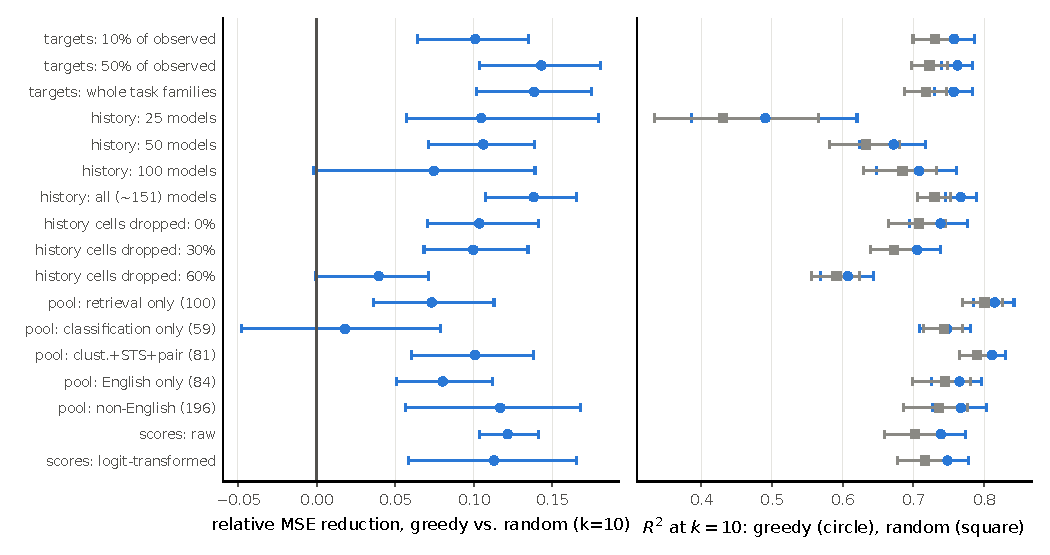
\includegraphics[width=\linewidth]{figs/conditions.pdf}
\caption{Data conditions (MTEB-main, $k=10$). Left: relative MSE reduction of greedy vs.\ random with 95\% CI. Right: $R^2$ of greedy (circle) and random (square).}
\label{fig:cond}
\end{figure}

\subsection{Theory against experiment}
\label{sec:exp_theory}
\begin{figure}[t]
\centering
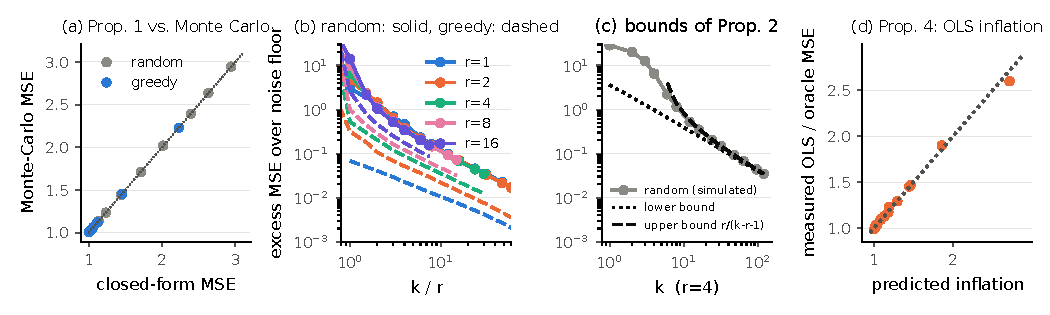
\includegraphics[width=\linewidth]{figs/synthetic_theory.pdf}
\caption{Synthetic checks. (a)~Prop.~\ref{prop:closed} vs.\ Monte Carlo. (b)~Excess error over the noise floor vs.\ $k/r$ ($N{=}400$, $g_i=10$): random-$S$ curves for different ranks collapse. (c)~Random-$S$ excess ($r=4$) between the bounds of Prop.~\ref{prop:random}. (d)~OLS/oracle MSE ratio vs.\ $1+k/(M-k-1)$ (Prop.~\ref{prop:ols}).}
\label{fig:synth}
\end{figure}
\emph{Synthetic factor models} (Fig.~\ref{fig:synth}). The closed form of Prop.~\ref{prop:closed} matches Monte Carlo to within 0.006 in MSE for all random and greedy sets tested. The sandwich of Prop.~\ref{prop:random} holds in all 94 (rank, strength, $k$) cells with $k\ge r+2$ (within 3 MC standard errors), and the smallest $k$ with simulated excess $\le\epsilon\sigma^2$ lies in $[r/\epsilon-1/g,\ r(1+1/\epsilon)+1]$ in 21 of 24 settings and exceeds the upper end by one (MC noise at the bound) in the other three: e.g.\ $r=8,\ \epsilon=0.1$ requires $k=90$, i.e.\ $\approx 11r$. Greedy selection reaches the same excess with 0.08--0.48 (median 0.29) times as many benchmarks (e.g.\ 38 instead of 90 for $r=8,\epsilon=0.1$), a far larger gain than on real matrices, whose spectra have one dominant factor that random sets already capture. The OLS inflation $1+k/(M-k-1)$ of Prop.~\ref{prop:ols} agrees with simulation to a mean absolute deviation of 0.016 (max.\ 4.3\% relative). The spectral bound of Prop.~\ref{prop:tail} is never violated by the exhaustive optimum (0 of 480 instances) and is on average 82\% of it. Greedy selection recovers 99.7\% of the variance reduction of the exhaustive optimum on average (min.\ 0.91, 480 small instances; random: 0.87; the Das--Kempe bound is $0.18$ on average, hence loose), and a swap local search from the greedy set improves the residual objective by 1.4\% on average (max.\ 13\%) at $N=60$. The gain of greedy over random depends on the structure as the theory suggests (Appendix Table~\ref{tab:e5}): at $k=8$ the reduction of the residual objective is 3--8\% for one factor, 4--16\% for two, 5--29\% for four and 10--57\% for eight; it grows with factor strength $g$ and rank $r$ and shrinks when leverage is heterogeneous (log-sd $\kappa$ of the loading scales).

\emph{Real matrices.} The error that the fitted Gaussian predicts for itself, $\mathrm{tr}(\Sigma_{T|S})/|T|$, tracks the held-out MSE closely for both selectors (Appendix Fig.~\ref{fig:calib}): its ratio to the held-out error averages 0.97 (MTEB-main), 0.89 (MTEB-dense), 1.10 (MTEB-eng), 1.07 (HELM-22), and 1.03 (OpenLLM), within 0.62--1.26 over all $k$ and matrices. The model-implied curve can therefore be used to \emph{plan} $k$ for a target accuracy before running anything. Prop.~\ref{prop:tail} bounds in-sample residuals of any selection from below (Appendix Fig.~\ref{fig:spectral}); the in-sample greedy residual is 1.2--1.6$\times$ the bound on MTEB-main for $k\le40$, while random selection is 1.5--2.0$\times$.


\subsection{A protocol pitfall: scoring the complement}
\label{sec:exp_pitfall}
A natural protocol lets each selector pick $S$ from \emph{all} observed benchmarks and scores the model on the \emph{remaining} $C\setminus S$. Then selectors are scored on different targets, and a rule that removes the hardest-to-explain benchmarks into $S$ leaves the easy ones as targets. Appendix Table~\ref{tab:bias} compares both protocols for the same selected sets. With complement targets greedy appears to beat random at $k=40$ on MTEB-main by a MSE of 0.18 vs.\ 0.23 and at $k=12$ on HELM-Lite-22 by 0.27 vs.\ 0.42; on fixed targets the advantage is nil (0.24 vs.\ 0.24 and 0.41 vs.\ 0.42). The inflation is largest exactly where the budget is large relative to $N$.


\section{Discussion and limitations}
\label{sec:disc}

\paragraph{What the evidence supports.}
(1)~A handful of well-chosen benchmarks gives most of what a larger budget would: on MTEB-main five tasks of $\sim$215 explain 71\% of the variance (relative to the mean baseline) of a new model's other scores, ten explain 76\%, and no budget up to 40 passes $\approx$80\%. (2)~The choice of benchmarks matters mainly below $k\approx10$ and the gain over random is substantial there (13--21\% in MSE), but it is not uniformly positive: it is absent for homogeneous pools and for $k$ comparable to the pool size, and it is negative for LiveBench-7 at $k=3$. (3)~Heuristics that look reasonable can hurt: the most-evaluated benchmarks are worse than random at every $k$ we tried on MTEB-main, and the most-correlated ones from $k=6$ on. (4)~The theory explains the shape: an irreducible per-benchmark floor, a requirement $k\gtrsim r(1+1/\epsilon)$ for a factor structure of rank $r$, and a spectral lower bound that no selection can beat; the sandwich and the finite-history inflation are accurate in simulation, and the fitted Gaussian predicts its own error on real matrices. The hypothesis that a small subset suffices to infer the rest is thus \emph{supported in the regime of moderate accuracy} (about 75\% of variance) and \emph{not supported for accurate prediction of individual scores}, where a plateau remains.

\paragraph{Where it fails or is unproven.}
\textbf{Plateau.} A residual of 20--30\% of variance is benchmark-specific; we do not know how much is evaluation noise and how much true specialization, so we cannot say whether more data or better predictors would remove it. \textbf{Gaussian linear model.} The mean-and-covariance model ignores ceiling effects and non-linear dependence; \textsc{kNN} beats it at $k=1$ by 5--8 points of $R^2$, and a logit transform gave no gain. The factor-model covariance, although natural for the theory, selected 5--9\% worse than the pairwise covariance at $k\ge10$, and low-rank prediction was never better than the full covariance: our theory is a guide to scaling, not a description of these matrices. \textbf{Selection is not adaptive.} Under the Gaussian model adaptivity gives nothing (Prop.~\ref{prop:closed}), but we did not test adaptive policies with non-Gaussian predictors. \textbf{Retrospective protocol.} A model's observed benchmarks are not random: authors choose where to report (missing not at random); we restrict selection to the model's observed set and score on its other observed benchmarks, which may flatter methods in either direction. Costs per benchmark are ignored; a cost-aware greedy ratio rule is a one-line change but untested. \textbf{Data.} MTEB models are text-embedding models, not generative LLMs; the three LLM matrices have $N\le22$, so $k$ cannot exceed 3--12 and conclusions about large budgets rest on MTEB alone. Near-duplicate models (merges, fine-tunes, sizes of one family) make random splits optimistic; the organisation and temporal splits reduce but do not remove this. The time split for MTEB has only 53 test models. The MTEB subset we use consists of tasks evaluated for $\ge$100 models, which over-represents widely run tasks. We tuned hyper-parameters on the training rows only, but chose \textsc{Gauss} as the default after looking at inner validation on MTEB-main, and the study designed its protocol after a first, flawed run with complement targets (\S\ref{sec:exp_pitfall}; that section reports a controlled re-run, not the first run). \textbf{Scope of the claims.} Statements about ``$k$ needed'' depend on the target accuracy, the matrix, and the shift between history and new model; they are not universal constants.

\paragraph{Practical guidance.} With a history like MTEB-main, run 5--10 benchmarks chosen by greedy variance reduction (or $k$-medoids), predict with the conditional Gaussian (\textsc{kNN} for $k=1$), expect the \emph{average} of the other scores to be within $\sim$1--2 points but individual scores only within $\sim$7--8, plan $k$ with the model-implied error, and re-check against full evaluations when the new model comes from a different lab or period.

\paragraph{Broader impact.} Cheaper evaluation saves energy and lowers entry barriers, but risks over-reliance on proxy benchmarks; inferred scores should be labelled as such.


\bibliographystyle{plainnat}
\bibliography{refs}

\appendix
\section{Proofs of the propositions}
\label{app:proofs}

Throughout, $z\sim\mathcal N(0,\Sigma)$ is standardized; $S$ is fixed before the data are seen (the posterior covariance below does not depend on the data, which is the content of the last claim of Prop.~\ref{prop:closed}).

\paragraph{Proof of Prop.~\ref{prop:closed}.}
Write $z=\Lambda f+\varepsilon$, $f\sim\mathcal N(0,I_r)$, $\varepsilon\sim\mathcal N(0,\Psi)$. Given $z_S$, $f\mid z_S\sim\mathcal N(m,P)$ with $P=(I+\Lambda_S^\top\Psi_S^{-1}\Lambda_S)^{-1}$ and $m=P\Lambda_S^\top\Psi_S^{-1}z_S$ (Gaussian conditioning). For $j\notin S$, $z_j=\lambda_j^\top f+\varepsilon_j$ with $\varepsilon_j$ independent of $(f,z_S)$, so the Bayes predictor is $\lambda_j^\top m$ and $\mathrm{Var}(z_j\mid z_S)=\psi_j+\lambda_j^\top P\lambda_j$. This equals $\Sigma_{jj}-\Sigma_{jS}\Sigma_{SS}^{-1}\Sigma_{Sj}$ by the Woodbury identity. Since $P\succeq0$, $v_j\ge\psi_j$. Adding an index $s$ to $S$ adds $\lambda_s\lambda_s^\top/\psi_s\succeq0$ to $P^{-1}$, hence lowers $P$ in the Loewner order and $v_j$ weakly decreases. $P$ is free of $z_S$, so for any (possibly adaptive) selection policy the conditional variance after $k$ steps is that of the set actually chosen; the expected error of an adaptive policy is an average of $v_j(S)$ over the sets it can produce, which is at least $\min_{|S|=k}v_j(S)$, attained by a non-adaptive set. \qed

\paragraph{Proof of Prop.~\ref{prop:random}.}
Let $W=\Lambda_S^\top\Lambda_S/\sigma^2=\sum_{s\in S}\tilde\lambda_s\tilde\lambda_s^\top$ with $\tilde\lambda_s\sim\mathcal N(0,G)$ i.i.d., i.e.\ $W\sim\mathrm{Wishart}_r(k,G)$, so $\mathbb{E}W=kG$, and for $k\ge r+2$, $\mathbb{E}W^{-1}=G^{-1}/(k-r-1)$. For the target $j\notin S$, $\lambda_j$ is independent of $S$ with $\mathbb{E}\lambda_j\lambda_j^\top=\sigma^2G$, hence $\mathbb{E}[v_j-\sigma^2]=\sigma^2\,\mathrm{tr}\big(G\,\mathbb{E}(I+W)^{-1}\big)$.
\emph{Lower bound:} $W\mapsto(I+W)^{-1}$ is operator convex, so $\mathbb{E}(I+W)^{-1}\succeq(I+kG)^{-1}$ and $\mathrm{tr}(G(I+kG)^{-1})=\sum_i g_i/(1+kg_i)$.
\emph{Upper bound:} $(I+W)^{-1}\preceq W^{-1}$ whenever $W\succ0$ (a.s.\ for $k\ge r$), so $\mathrm{tr}(G\,\mathbb{E}W^{-1})=r/(k-r-1)$.
For $g_i\equiv g$: the lower bound is $rg/(1+kg)\le\epsilon$ iff $k\ge r/\epsilon-1/g$, and the upper bound is $\le\epsilon$ iff $k\ge r+1+r/\epsilon$. \qed

\paragraph{Proof of Prop.~\ref{prop:tail}.}
$\Sigma_{\cdot\mid S}=\Sigma-B$ with $B=\Sigma_{\cdot S}\Sigma_{SS}^{-1}\Sigma_{S\cdot}\succeq0$ of rank $\le k$ and $F(S)=\mathrm{tr}(\Sigma-B)$. By Weyl's inequality, $\lambda_{i+k}(\Sigma)\le\lambda_i(\Sigma-B)+\lambda_{k+1}(B)=\lambda_i(\Sigma-B)$, so $\mathrm{tr}(\Sigma-B)\ge\sum_{i\ge1}\lambda_{i+k}(\Sigma)$. For $\Sigma=\Lambda\Lambda^\top+\sigma^2I$ with $\mathrm{rank}\,\Lambda=r$, $\lambda_i(\Sigma)=\sigma^2$ for $i>r$, so for $k\ge r$ the sum is $(N-k)\sigma^2$. \qed

\paragraph{Proof of Prop.~\ref{prop:ols}.}
Under Gaussianity, $z_j=\beta^\top z_S+e$ with $e\sim\mathcal N(0,s^2)$ independent of $z_S$ and $s^2=v_j(S)$. With $X_S\in\mathbb{R}^{M\times k}$ the training design, $\hat\beta-\beta\mid X_S\sim\mathcal N(0,s^2(X_S^\top X_S)^{-1})$. For a fresh $z_S$, $\mathbb{E}(\hat\beta^\top z_S-z_j)^2=s^2+\mathbb{E}\,z_S^\top(\hat\beta-\beta)(\hat\beta-\beta)^\top z_S=s^2\big(1+\mathrm{tr}(\Sigma_{SS}\,\mathbb{E}(X_S^\top X_S)^{-1})\big)$. As $X_S^\top X_S\sim\mathrm{Wishart}_k(M,\Sigma_{SS})$, $\mathbb{E}(X_S^\top X_S)^{-1}=\Sigma_{SS}^{-1}/(M-k-1)$, giving $s^2(1+k/(M-k-1))$. \qed

\paragraph{On the greedy guarantee.}
$f(S)=\sum_j\mathrm{Var}(z_j)R_j^2(S)$ with $R^2_j(S)=1-v_j(S)/\Sigma_{jj}$ (equal to $1$ if $j\in S$). \citet{das2011submodular} show that the objective $R^2(y;z_S)$ of selecting $S$ to linearly predict a single variable $y$ has submodularity ratio $\gamma\ge\lambda_{\min}(C)$, $C$ the correlation matrix of the candidates, and that greedy forward selection attains at least $(1-e^{-\gamma})$ of the optimum. The submodularity ratio of a non-negative combination of monotone set functions is at least the minimum of the ratios, so the same bound holds for $f$ (we rely on their theorem for the single-target case and do not re-derive it). Under the factor model $\lambda_{\min}(C)\ge\min_j\psi_j/\Sigma_{jj}$ (since $\Sigma\succeq\Psi$), which is small whenever some benchmark is nearly explained by the others; the guarantee is then loose, and the empirical check of \S\ref{sec:exp_theory} is the operative evidence.

\section{Further experimental details and tables}
\label{app:details}

\subsection{Implementation details}
\label{app:impl}
\textbf{Standardization.} Per benchmark, with training-row mean and standard deviation (observed cells only). Errors are always reported on the standardized scale (``MSE'') and, where stated, in score points; $R^2=1-\mathrm{MSE}/\mathrm{MSE}_{\textsc{mean}}$ with $\textsc{mean}$ the training-mean predictor on the same targets (its standardized MSE exceeds 1 because held-out models differ systematically from the history: 1.18 on random splits, 1.36 for new organisations, 3.25 for later releases, MTEB-main).
\textbf{Covariance.} Pairwise-complete correlation with $\ge5$ co-observed models per pair (else 0), eigenvalues clipped at $10^{-3}$ and rescaled to unit diagonal, then $\Sigma_\kappa=(1-\kappa)\hat C+\kappa I$ with $\kappa\in\{0,0.05,0.15,0.3,0.5\}$ chosen on an inner split (20\% of training rows as validation models; for each, a random half of its observed benchmarks (at most 10) plays $S$, the rest targets). The same inner split tunes FA rank $r\in\{1,2,3,4,6,8,12\}$ (restricted to $(N-r)^2>N+r$), ISVD rank/ridge, $K$ of \textsc{kNN} ($\{5,15,40\}$) and the \textsc{Hybrid} blend; \textsc{Gauss} was selected for the main pipeline \emph{because} it did best in that inner validation on MTEB-main.
\textbf{FA by EM} uses the missing-data E-step (per-row posterior over observed benchmarks), a small ridge on loadings (0.05), and a floor $\psi_j\ge0.02$ on unique variances; 300 iterations at most.
\textbf{Selectors.} \textsc{Greedy} is Eq.~\eqref{eq:greedy}; \textsc{Greedy-MI} maximizes $\mathrm{Var}(z_j\mid z_S)\,(\Sigma^{-1})_{jj}$ (the criterion of \citet{krause2008near} simplifies since $\mathrm{Var}(z_j\mid\text{all others})=1/(\Sigma^{-1})_{jj}$ does not depend on $S$); \textsc{$k$-medoids}: 5 $k$-means++-seeded restarts on $1-|\rho_{ij}|$, medoids are not nested in $k$; ``top-SNR'' ranks by factor-model communality over unique variance. ``Most-evaluated'' orders benchmarks by their number of training observations (ties by column order).
\textbf{Held-out targets.} $T_0$ is a random 30\% of the model's observed set (at least 2) with two draws per model for MTEB, four for HELM-22 (pool sizes: up to $\sim$195 on MTEB-main); for $N\le12$ the held-out target is each benchmark in turn. We evaluate $k\le0.7\,|C|-3$ roughly, capped at 40 (14 for HELM-22; $\min_i|C_i|-2$ for $N\le12$). A (model, target-draw) cell is used in a curve only if it is available for every $k$ of that curve.
\textbf{Aggregation.} For each (selector, predictor, $k$), values are averaged over random draws and cells, then over repeats/folds per model; the bootstrap resamples models (2000 replicates, seed fixed).

\subsection{Reproducibility}
\label{app:repro}
Code, the processed matrices' construction scripts, and a README with commands, seeds, timings and the script that generates every table and figure are in the supplementary archive.
\textbf{Pinned data:} MTEB results repository at commit \texttt{6dabbcc6} (CC0-1.0); Open LLM Leaderboard \texttt{contents} at \texttt{9c09a7ca} (no explicit license; 4,576 rows, we drop 80 flagged or duplicate model entries); HELM Lite release v1.13.0 (\texttt{core\_scenarios}, \texttt{mmlu}, \texttt{legalbench}, \texttt{wmt\_14} group files); LiveBench \texttt{model\_judgment} at \texttt{9704e5da} (a 7-task per-model summary; mean of per-question scores per model and task $\times100$). MTEB task types and languages come from the \texttt{mteb} package (v2.26.31; used only for task metadata, 958 of the 1,172 tasks matched; the others are typed by name). One MTEB score is the \texttt{main\_score} of the test split (validation or dev if no test split), averaged over language subsets; tasks with differing subset sets across models keep only the modal one; tasks with scores outside $[-100,100]$ (two hardware-speed tasks) are dropped.
\textbf{Compute:} CPU only (40 cores, 250 GB RAM, of which a few GB used). The full pipeline (\texttt{run\_everything.sh}: synthetic checks, all real-data runs, ablations, tables) took about 1.1 h wall-clock; the second stage ran up to $\sim$80 processes on the 40 cores, so the summed per-fold wall times (22.7 h) overstate CPU time; one MTEB-main random-split fold (tuning of 6 predictors + all selectors) takes $\approx$ 8 min on one core when the machine is not oversubscribed, the synthetic checks $\approx$ 5 min. Data: 3.4 GB for the cloned MTEB repository (extracted matrices: a few MB).

\subsection{Additional results}
\label{app:more}

\begin{figure}[h]
\centering
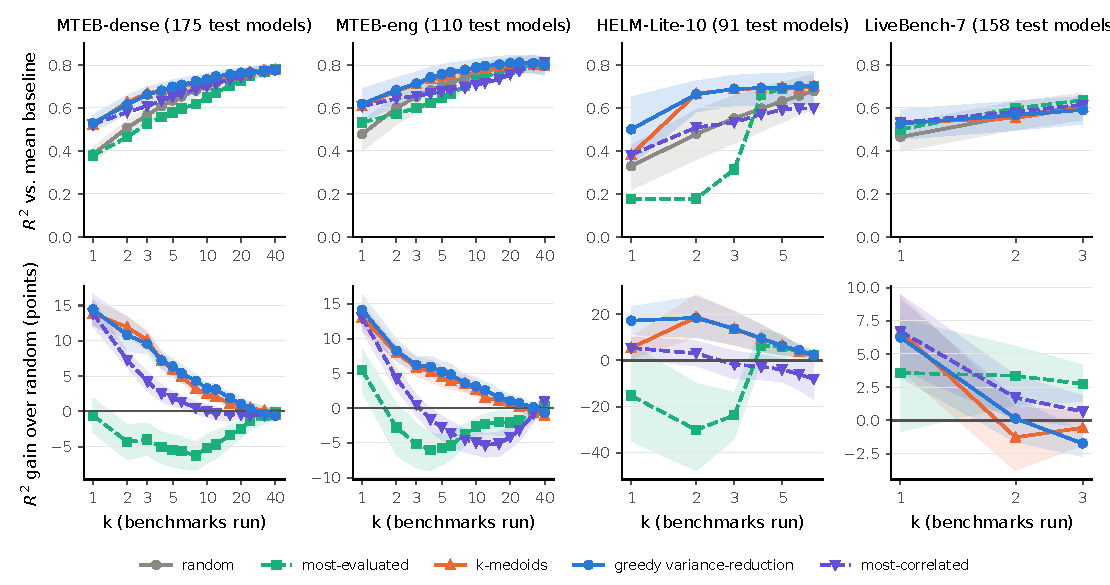
\includegraphics[width=\linewidth]{figs/curves_appendix.pdf}
\caption{As Fig.~\ref{fig:main} for the other matrices (random splits), with the most-correlated selector added. HELM-Lite-10 and LiveBench-7 have complete or nearly complete pools; the number of test models is the number of held-out models that have all budgets available.}
\label{fig:app_curves}
\end{figure}

\begin{table}[h]
\centering\small
\caption{Predictors on MTEB-main ($R^2$; random splits). 95\% CIs of $\pm$0.03--0.04 for each cell; paired differences in Appendix Table~\ref{tab:ci_pred}.}
\label{tab:pred}
\begin{tabular}{llccccc}\toprule
Selection & Predictor & $k{=}1$ & $k{=}5$ & $k{=}10$ & $k{=}20$ & $k{=}40$ \\\midrule
random & AvgShift & 0.40 & 0.55 & 0.58 & 0.60 & 0.61 \\
 & kNN & 0.45 & 0.67 & 0.74 & 0.77 & 0.78 \\
 & ISVD & 0.40 & 0.64 & 0.70 & 0.74 & 0.77 \\
 & FA & 0.38 & 0.65 & 0.71 & 0.76 & 0.78 \\
 & Gauss & 0.39 & 0.65 & 0.72 & 0.77 & 0.80 \\
 & Hybrid & 0.39 & 0.65 & 0.72 & 0.77 & 0.82 \\
\midrule
greedy variance-reduction & AvgShift & 0.53 & 0.58 & 0.59 & 0.59 & 0.60 \\
 & kNN & 0.60 & 0.70 & 0.75 & 0.77 & 0.78 \\
 & ISVD & 0.53 & 0.69 & 0.74 & 0.75 & 0.76 \\
 & FA & 0.54 & 0.71 & 0.75 & 0.77 & 0.79 \\
 & Gauss & 0.52 & 0.71 & 0.76 & 0.79 & 0.80 \\
 & Hybrid & 0.52 & 0.71 & 0.76 & 0.80 & 0.82 \\
\bottomrule
\end{tabular}

\end{table}

\begin{table}[h]
\centering\small
\caption{Standardized MSE under fixed held-out targets $T_0$ (this paper) vs.\ complement targets $C\setminus S$ (naive).}
\label{tab:bias}
\resizebox{\linewidth}{!}{\begin{tabular}{lllccc}\toprule
Dataset & Targets & Selector & small $k$ & mid $k$ & large $k$ \\\midrule
HELM-Lite-22 ($k{=}2,5,12$) & fixed $T_0$ & random & 0.67 & 0.54 & 0.42 \\
HELM-Lite-22 ($k{=}2,5,12$) & fixed $T_0$ & greedy variance-reduction & 0.63 & 0.48 & 0.41 \\
HELM-Lite-22 ($k{=}2,5,12$) & complement $C\!\setminus\!S$ & random & 0.66 & 0.48 & 0.42 \\
HELM-Lite-22 ($k{=}2,5,12$) & complement $C\!\setminus\!S$ & greedy variance-reduction & 0.61 & 0.42 & 0.27 \\
\midrule
MTEB-main ($k{=}2,10,40$) & fixed $T_0$ & random & 0.57 & 0.34 & 0.24 \\
MTEB-main ($k{=}2,10,40$) & fixed $T_0$ & greedy variance-reduction & 0.47 & 0.29 & 0.24 \\
MTEB-main ($k{=}2,10,40$) & complement $C\!\setminus\!S$ & random & 0.55 & 0.33 & 0.23 \\
MTEB-main ($k{=}2,10,40$) & complement $C\!\setminus\!S$ & greedy variance-reduction & 0.45 & 0.27 & 0.18 \\
\bottomrule
\end{tabular}
}
\end{table}


\begin{table}[h]
\centering\small
\caption{As Table~\ref{tab:main} for the other matrices.}
\label{tab:main_app}
\resizebox{\linewidth}{!}{\begin{tabular}{llcccc}\toprule
Dataset (split) & Selector & $k{=}1$ & $k{=}3$ & $k{=}5$ & $k{=}10$ \\\midrule
MTEB-dense (rand) & random & 0.38 \scriptsize[0.35,0.42] & 0.57 \scriptsize[0.53,0.60] & 0.63 \scriptsize[0.60,0.67] & 0.70 \scriptsize[0.67,0.73] \\
 & most-evaluated & 0.38 \scriptsize[0.34,0.42] & 0.53 \scriptsize[0.49,0.57] & 0.58 \scriptsize[0.54,0.61] & 0.65 \scriptsize[0.62,0.68] \\
 & k-medoids & 0.52 \scriptsize[0.48,0.56] & \textbf{0.67} \scriptsize[0.63,0.70] & 0.69 \scriptsize[0.66,0.72] & \textbf{0.73} \scriptsize[0.69,0.75] \\
 & greedy variance-reduction & \textbf{0.53} \scriptsize[0.49,0.57] & 0.66 \scriptsize[0.62,0.70] & \textbf{0.70} \scriptsize[0.66,0.73] & \textbf{0.73} \scriptsize[0.70,0.76] \\
\midrule
MTEB-eng (rand) & random & 0.48 \scriptsize[0.40,0.54] & 0.65 \scriptsize[0.58,0.71] & 0.70 \scriptsize[0.64,0.76] & 0.76 \scriptsize[0.70,0.80] \\
 & most-evaluated & 0.53 \scriptsize[0.45,0.60] & 0.60 \scriptsize[0.52,0.66] & 0.65 \scriptsize[0.58,0.70] & 0.73 \scriptsize[0.67,0.78] \\
 & k-medoids & 0.61 \scriptsize[0.53,0.67] & \textbf{0.71} \scriptsize[0.64,0.76] & 0.75 \scriptsize[0.69,0.79] & 0.78 \scriptsize[0.73,0.82] \\
 & greedy variance-reduction & \textbf{0.62} \scriptsize[0.53,0.69] & \textbf{0.71} \scriptsize[0.64,0.77] & \textbf{0.76} \scriptsize[0.70,0.80] & \textbf{0.79} \scriptsize[0.74,0.83] \\
\midrule
HELM-Lite-10 (rand) & random & 0.33 \scriptsize[0.22,0.43] & 0.55 \scriptsize[0.44,0.66] & 0.63 \scriptsize[0.53,0.72] & -- \\
 & most-evaluated & 0.18 \scriptsize[0.06,0.30] & 0.31 \scriptsize[0.23,0.39] & 0.69 \scriptsize[0.62,0.75] & -- \\
 & k-medoids & 0.38 \scriptsize[0.24,0.51] & \textbf{0.69} \scriptsize[0.61,0.75] & \textbf{0.70} \scriptsize[0.62,0.76] & -- \\
 & greedy variance-reduction & \textbf{0.50} \scriptsize[0.34,0.65] & \textbf{0.69} \scriptsize[0.61,0.75] & 0.69 \scriptsize[0.61,0.76] & -- \\
\bottomrule
\end{tabular}
}
\end{table}

\begin{table}[h]
\centering\scriptsize
\caption{Predictors on MTEB-main: paired difference $R^2_{\text{predictor}}-R^2_{\textsc{Gauss}}$ with 95\% bootstrap CI (positive = better than \textsc{Gauss}); the \textsc{Gauss} rows show its own $R^2$ [95\% CI].}
\label{tab:ci_pred}
{\tiny\setlength{\tabcolsep}{2pt}\begin{tabular}{llccccc}\toprule
Selection & Predictor & $k{=}1$ & $k{=}5$ & $k{=}10$ & $k{=}20$ & $k{=}40$ \\\midrule
random & AvgShift & +0.004 [+0.002,+0.006] & -0.099 [-0.113,-0.087] & -0.136 [-0.154,-0.121] & -0.168 [-0.188,-0.151] & -0.193 [-0.215,-0.173] \\
 & kNN & +0.053 [+0.030,+0.071] & +0.015 [-0.000,+0.029] & +0.018 [-0.001,+0.034] & -0.004 [-0.024,+0.014] & -0.021 [-0.042,-0.000] \\
 & ISVD & +0.003 [-0.009,+0.015] & -0.012 [-0.020,-0.005] & -0.020 [-0.028,-0.013] & -0.029 [-0.036,-0.022] & -0.036 [-0.045,-0.028] \\
 & FA & -0.009 [-0.019,+0.000] & -0.002 [-0.008,+0.004] & -0.007 [-0.013,-0.002] & -0.013 [-0.019,-0.007] & -0.021 [-0.031,-0.010] \\
 & Gauss & 0.394 [0.361,0.423] & 0.652 [0.618,0.684] & 0.720 [0.690,0.749] & 0.769 [0.743,0.793] & 0.802 [0.781,0.823] \\
 & Hybrid & -0.004 [-0.006,-0.002] & +0.001 [-0.001,+0.002] & +0.002 [+0.001,+0.004] & +0.005 [+0.003,+0.008] & +0.013 [+0.010,+0.018] \\
\midrule
greedy variance-reduction & AvgShift & +0.005 [+0.002,+0.008] & -0.128 [-0.146,-0.112] & -0.166 [-0.188,-0.146] & -0.199 [-0.233,-0.172] & -0.201 [-0.227,-0.177] \\
 & kNN & +0.075 [+0.047,+0.100] & -0.007 [-0.030,+0.014] & -0.010 [-0.034,+0.012] & -0.021 [-0.043,+0.001] & -0.020 [-0.043,+0.002] \\
 & ISVD & +0.006 [-0.004,+0.018] & -0.018 [-0.030,-0.008] & -0.023 [-0.032,-0.014] & -0.037 [-0.045,-0.030] & -0.036 [-0.044,-0.027] \\
 & FA & +0.018 [+0.006,+0.029] & +0.000 [-0.010,+0.010] & -0.007 [-0.016,+0.001] & -0.015 [-0.025,-0.005] & -0.013 [-0.027,+0.001] \\
 & Gauss & 0.520 [0.479,0.559] & 0.709 [0.676,0.741] & 0.758 [0.733,0.781] & 0.788 [0.767,0.809] & 0.800 [0.778,0.820] \\
 & Hybrid & -0.003 [-0.005,-0.001] & +0.002 [+0.001,+0.004] & +0.004 [+0.002,+0.006] & +0.010 [+0.007,+0.012] & +0.023 [+0.018,+0.029] \\
\bottomrule
\end{tabular}
}
\end{table}

\begin{table}[h]
\centering\small
\caption{Where the selection covariance comes from: relative MSE reduction (\%, with CI) of greedy selection using the covariance of all rows including test models (``oracle''), or the rank-$r$ factor-model covariance, over our default (pairwise covariance from training rows). Positive = better than default.}
\label{tab:oracle}
\resizebox{\linewidth}{!}{\begin{tabular}{llccccc}\toprule
Dataset & Selection covariance & $k{=}1$ & $k{=}3$ & $k{=}5$ & $k{=}10$ & $k{=}20$ \\\midrule
MTEB-main & oracle covariance & +1.0\,[+0.1,+1.9] & +2.6\,[+1.1,+4.0] & +3.8\,[+1.2,+6.7] & +2.6\,[+1.3,+3.9] & +0.8\,[-3.6,+3.9] \\
MTEB-main & FA covariance & +0.2\,[-3.4,+3.7] & -1.5\,[-4.6,+1.1] & -2.5\,[-5.2,-0.2] & -5.3\,[-8.3,-2.1] & -9.4\,[-13.8,-5.9] \\
MTEB-dense & oracle covariance & +1.6\,[+0.0,+3.2] & +3.0\,[+0.8,+5.3] & +2.1\,[+0.1,+4.3] & +1.8\,[-0.6,+4.1] & +0.4\,[-2.0,+2.6] \\
MTEB-dense & FA covariance & -0.6\,[-3.8,+1.9] & -2.2\,[-5.1,+0.4] & -1.3\,[-4.2,+1.2] & +0.6\,[-1.3,+2.6] & -4.0\,[-6.1,-1.7] \\
MTEB-eng & oracle covariance & +3.6\,[+1.1,+6.6] & +4.6\,[+1.8,+7.4] & +3.8\,[+1.2,+6.4] & +1.3\,[-1.2,+3.7] & +0.3\,[-1.7,+2.4] \\
MTEB-eng & FA covariance & +1.1\,[-6.1,+7.5] & -6.5\,[-10.7,-2.6] & +1.2\,[-2.5,+4.8] & +2.8\,[-0.3,+5.9] & +0.2\,[-1.9,+2.3] \\
HELM-Lite-22 & oracle covariance & +2.3\,[+0.6,+4.8] & +3.6\,[+0.6,+6.8] & +0.9\,[-0.4,+2.4] & +0.9\,[-0.0,+1.9] & -- \\
HELM-Lite-22 & FA covariance & +0.5\,[-0.7,+1.9] & -0.9\,[-2.8,+0.9] & -0.9\,[-2.6,+0.8] & -0.2\,[-1.2,+0.6] & -- \\
\bottomrule
\end{tabular}
}
\end{table}

\begin{table}[h]
\centering\small
\caption{Synthetic factor models, $N=100$, $k=8$: relative reduction of the objective $F$ by greedy selection vs.\ random selection, by rank $r$, factor strength $g$ (per-benchmark SNR of each factor) and leverage heterogeneity $\kappa$ (log-sd of loading scales).}
\label{tab:e5}
\begin{tabular}{rrcccc}\toprule
$r$ & $g$ & $\kappa{=}0$ & $\kappa{=}0.5$ & $\kappa{=}1$ & $\kappa{=}1.5$ \\\midrule
1 & 0.3 & 3\% & 4\% & 4\% & 3\% \\
1 & 1 & 5\% & 6\% & 6\% & 4\% \\
1 & 3 & 8\% & 8\% & 7\% & 6\% \\
2 & 0.3 & 8\% & 8\% & 7\% & 4\% \\
2 & 1 & 12\% & 12\% & 10\% & 7\% \\
2 & 3 & 16\% & 16\% & 13\% & 9\% \\
4 & 0.3 & 15\% & 14\% & 9\% & 5\% \\
4 & 1 & 24\% & 22\% & 16\% & 9\% \\
4 & 3 & 29\% & 28\% & 21\% & 13\% \\
8 & 0.3 & 24\% & 23\% & 16\% & 10\% \\
8 & 1 & 45\% & 40\% & 28\% & 17\% \\
8 & 3 & 57\% & 54\% & 38\% & 25\% \\
\bottomrule
\end{tabular}

\end{table}

\begin{table}[h]
\centering\small
\caption{First twelve benchmarks chosen by the greedy rule on the full MTEB-main correlation matrix (illustration, in-sample), and the residual variance per benchmark they leave. The first pick is a multilingual retrieval task, followed by English retrieval, classification and STS: the rule spreads its picks over families rather than over one type.}
\label{tab:picks}
\begin{tabular}{rllr}\toprule
$j$ & Task & Type / languages & resid.\ var. \\\midrule
1 & BelebeleRetrieval & Retrieval / acm,afr,als... & 0.55 \\
2 & CQADupstackPhysicsRetrieval & Retrieval / eng & 0.43 \\
3 & AngryTweetsClassification & Classification / unk & 0.38 \\
4 & STS14 & STS / eng & 0.36 \\
5 & CyrillicTurkicLangClassification & Classification / bak,chv,kaz... & 0.34 \\
6 & TempReasonL2Fact & Retrieval / eng & 0.32 \\
7 & KorSTS & STS / kor & 0.31 \\
8 & LEMBQMSumRetrieval & Retrieval / eng & 0.30 \\
9 & PSC & PairClassification / pol & 0.29 \\
10 & NusaParagraphEmotionClassification & Classification / bbc,bew,bug... & 0.27 \\
11 & RUParaPhraserSTS & STS / rus & 0.27 \\
12 & MedrxivClusteringS2S.v2 & Clustering / eng & 0.26 \\
\bottomrule\end{tabular}

\end{table}

\begin{figure}[h]
\centering
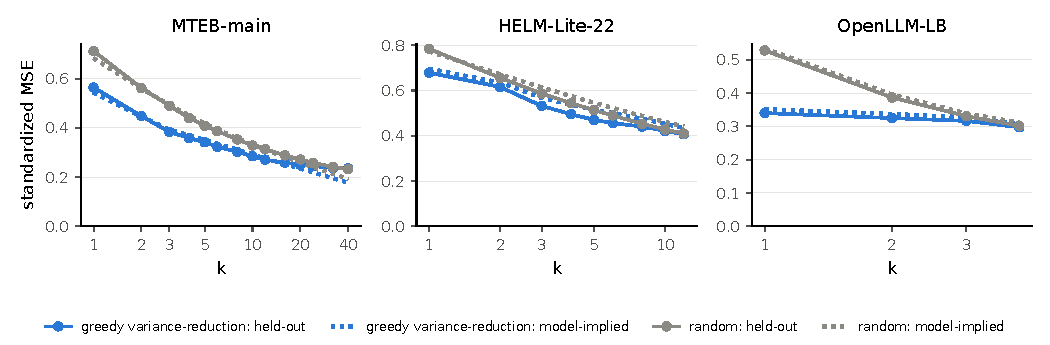
\includegraphics[width=\linewidth]{figs/calibration.pdf}
\caption{Model-implied expected MSE (dotted) vs.\ held-out MSE (solid) for greedy and random selection.}
\label{fig:calib}
\end{figure}

\begin{figure}[h]
\centering
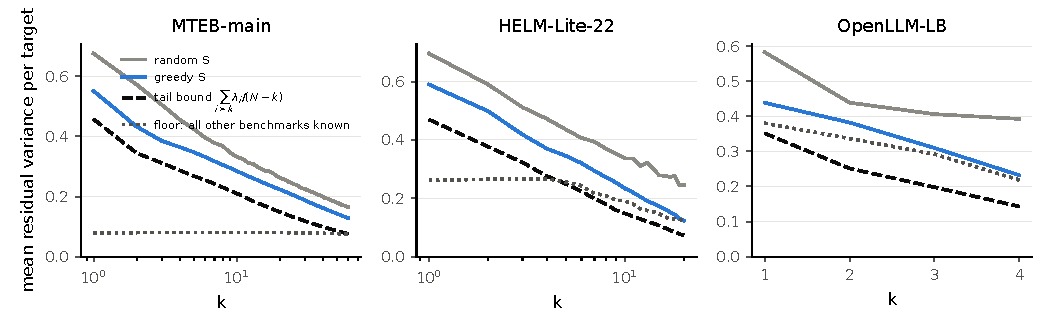
\includegraphics[width=\linewidth]{figs/spectral.pdf}
\caption{In-sample view on the full matrices (pairwise correlation matrix, light shrinkage): mean residual variance per remaining benchmark for random and greedy sets, the spectral tail bound of Prop.~\ref{prop:tail}, and the floor if all other benchmarks were known. Greedy sits between random and the bound.}
\label{fig:spectral}
\end{figure}

\paragraph{Aggregate error.} Mean absolute error (score points) of the \emph{average} of the held-out scores of a model (MTEB-main, \textsc{Gauss}, random splits; 95\% bootstrap CI): greedy 3.8 [3.5, 4.2] at $k=1$, 2.1 [1.9, 2.3] at 3, 1.7 [1.6, 1.9] at 5, 1.3 [1.2, 1.4] at 10, 1.1 [1.0, 1.2] at 20; random 6.2 [5.9, 6.5], 3.7 [3.5, 3.8], 2.7 [2.6, 2.8], 1.8 [1.7, 1.9], 1.3 [1.2, 1.4]; mean baseline 10.5. The RMSE per individual held-out benchmark is 11.0, 8.7, 8.0, 7.2, 6.9 (greedy) and 17.4 (baseline).

\paragraph{Ranking quality.} The per-benchmark Spearman correlation between predicted and actual scores across held-out models (MTEB-main, \textsc{Gauss}; average over benchmark$\times$fold pairs with $\ge8$ models) is 0.79/0.81/0.82 for greedy and 0.76/0.78/0.81 for random selection at $k=5/10/20$; MTEB-dense 0.77/0.78/0.79 vs.\ 0.73/0.77/0.79; HELM-Lite-22 0.71/0.72 vs.\ 0.68/0.74 at $k=5/10$. Models are therefore ranked well on any single benchmark with a handful of runs, and selection helps ranking less than it helps error.

\paragraph{Stability of the selected sets.} Running the greedy rule on each of the 15 training folds of the MTEB-main random splits (all 280 tasks as candidates, default shrinkage 0.05), the selected sets overlap only moderately: mean pairwise Jaccard similarity 0.23, 0.26, 0.26 at $k=5,10,20$ (a random set would give 0.01, 0.02, 0.04), because many tasks are near-substitutes. The most frequent first-ten picks are CyrillicTurkicLangClassification (13 of 15 folds), STS14 (12), TempReasonL2Fact (10), CQADupstackPhysicsRetrieval (10), AngryTweetsClassification (8) and BelebeleRetrieval (8). A practitioner should therefore treat the greedy list as one of many near-equivalent good subsets.

\paragraph{Number of models in the evaluation.} After requiring all budgets to be available for a cell, MTEB-main random splits use 189 models and 1,134 (model, fold, target-draw) cells, MTEB-main time-split 53 models; MTEB-eng 110 models; OpenLLM 4,496 (random) and 1,332 (temporal); HELM 91; LiveBench 158 in the first-3 budgets.


\section*{NeurIPS Paper Checklist}




\begin{enumerate}

\item {\bf Claims}
    \item[] Question: Do the main claims made in the abstract and introduction accurately reflect the paper's contributions and scope?
    \item[] Answer: \answerYes{}
    \item[] Justification: Abstract and Introduction state the method, theory and the empirical findings with their scope; \S\ref{sec:exp} reports every number cited there and \S\ref{sec:disc} states where the claims do not hold.
    \item[] Guidelines:
    \begin{itemize}
        \item The answer \answerNA{} means that the abstract and introduction do not include the claims made in the paper.
        \item The abstract and/or introduction should clearly state the claims made, including the contributions made in the paper and important assumptions and limitations. A \answerNo{} or \answerNA{} answer to this question will not be perceived well by the reviewers. 
        \item The claims made should match theoretical and experimental results, and reflect how much the results can be expected to generalize to other settings. 
        \item It is fine to include aspirational goals as motivation as long as it is clear that these goals are not attained by the paper. 
    \end{itemize}

\item {\bf Limitations}
    \item[] Question: Does the paper discuss the limitations of the work performed by the authors?
    \item[] Answer: \answerYes{}
    \item[] Justification: \S\ref{sec:disc} (``Where it fails or is unproven'') lists the modelling, protocol and data limitations; the Gaussian assumption, MTEB-only large-$N$ evidence and non-random missingness are discussed.
    \item[] Guidelines:
    \begin{itemize}
        \item The answer \answerNA{} means that the paper has no limitation while the answer \answerNo{} means that the paper has limitations, but those are not discussed in the paper. 
        \item The authors are encouraged to create a separate ``Limitations'' section in their paper.
        \item The paper should point out any strong assumptions and how robust the results are to violations of these assumptions (e.g., independence assumptions, noiseless settings, model well-specification, asymptotic approximations only holding locally). The authors should reflect on how these assumptions might be violated in practice and what the implications would be.
        \item The authors should reflect on the scope of the claims made, e.g., if the approach was only tested on a few datasets or with a few runs. In general, empirical results often depend on implicit assumptions, which should be articulated.
        \item The authors should reflect on the factors that influence the performance of the approach. For example, a facial recognition algorithm may perform poorly when image resolution is low or images are taken in low lighting. Or a speech-to-text system might not be used reliably to provide closed captions for online lectures because it fails to handle technical jargon.
        \item The authors should discuss the computational efficiency of the proposed algorithms and how they scale with dataset size.
        \item If applicable, the authors should discuss possible limitations of their approach to address problems of privacy and fairness.
        \item While the authors might fear that complete honesty about limitations might be used by reviewers as grounds for rejection, a worse outcome might be that reviewers discover limitations that aren't acknowledged in the paper. The authors should use their best judgment and recognize that individual actions in favor of transparency play an important role in developing norms that preserve the integrity of the community. Reviewers will be specifically instructed to not penalize honesty concerning limitations.
    \end{itemize}

\item {\bf Theory assumptions and proofs}
    \item[] Question: For each theoretical result, does the paper provide the full set of assumptions and a complete (and correct) proof?
    \item[] Answer: \answerYes{}
    \item[] Justification: Assumptions are stated in each proposition (\S\ref{sec:theory}); proofs are in Appendix~\ref{app:proofs}. The greedy approximation guarantee relies on a cited theorem (not re-derived) and is flagged as loose.
    \item[] Guidelines:
    \begin{itemize}
        \item The answer \answerNA{} means that the paper does not include theoretical results. 
        \item All the theorems, formulas, and proofs in the paper should be numbered and cross-referenced.
        \item All assumptions should be clearly stated or referenced in the statement of any theorems.
        \item The proofs can either appear in the main paper or the supplemental material, but if they appear in the supplemental material, the authors are encouraged to provide a short proof sketch to provide intuition. 
        \item Inversely, any informal proof provided in the core of the paper should be complemented by formal proofs provided in appendix or supplemental material.
        \item Theorems and Lemmas that the proof relies upon should be properly referenced. 
    \end{itemize}

    \item {\bf Experimental result reproducibility}
    \item[] Question: Does the paper fully disclose all the information needed to reproduce the main experimental results of the paper to the extent that it affects the main claims and/or conclusions of the paper (regardless of whether the code and data are provided or not)?
    \item[] Answer: \answerYes{}
    \item[] Justification: \S\ref{sec:exp}, Appendix~\ref{app:impl} and \ref{app:repro} describe data versions, preprocessing, splits, tuning, selectors and predictors; the supplementary README lists commands and seeds.
    \item[] Guidelines:
    \begin{itemize}
        \item The answer \answerNA{} means that the paper does not include experiments.
        \item If the paper includes experiments, a \answerNo{} answer to this question will not be perceived well by the reviewers: Making the paper reproducible is important, regardless of whether the code and data are provided or not.
        \item If the contribution is a dataset and\slash or model, the authors should describe the steps taken to make their results reproducible or verifiable. 
        \item Depending on the contribution, reproducibility can be accomplished in various ways. For example, if the contribution is a novel architecture, describing the architecture fully might suffice, or if the contribution is a specific model and empirical evaluation, it may be necessary to either make it possible for others to replicate the model with the same dataset, or provide access to the model. In general. releasing code and data is often one good way to accomplish this, but reproducibility can also be provided via detailed instructions for how to replicate the results, access to a hosted model (e.g., in the case of a large language model), releasing of a model checkpoint, or other means that are appropriate to the research performed.
        \item While NeurIPS does not require releasing code, the conference does require all submissions to provide some reasonable avenue for reproducibility, which may depend on the nature of the contribution. For example
        \begin{enumerate}
            \item If the contribution is primarily a new algorithm, the paper should make it clear how to reproduce that algorithm.
            \item If the contribution is primarily a new model architecture, the paper should describe the architecture clearly and fully.
            \item If the contribution is a new model (e.g., a large language model), then there should either be a way to access this model for reproducing the results or a way to reproduce the model (e.g., with an open-source dataset or instructions for how to construct the dataset).
            \item We recognize that reproducibility may be tricky in some cases, in which case authors are welcome to describe the particular way they provide for reproducibility. In the case of closed-source models, it may be that access to the model is limited in some way (e.g., to registered users), but it should be possible for other researchers to have some path to reproducing or verifying the results.
        \end{enumerate}
    \end{itemize}


\item {\bf Open access to data and code}
    \item[] Question: Does the paper provide open access to the data and code, with sufficient instructions to faithfully reproduce the main experimental results, as described in supplemental material?
    \item[] Answer: \answerYes{}
    \item[] Justification: All data are public and version-pinned (Appendix~\ref{app:repro}); the supplementary archive contains all code, a README with environment, commands, expected run times and a table mapping every figure/table to its script.
    \item[] Guidelines:
    \begin{itemize}
        \item The answer \answerNA{} means that paper does not include experiments requiring code.
        \item Please see the NeurIPS code and data submission guidelines (\url{https://neurips.cc/public/guides/CodeSubmissionPolicy}) for more details.
        \item While we encourage the release of code and data, we understand that this might not be possible, so \answerNo{} is an acceptable answer. Papers cannot be rejected simply for not including code, unless this is central to the contribution (e.g., for a new open-source benchmark).
        \item The instructions should contain the exact command and environment needed to run to reproduce the results. See the NeurIPS code and data submission guidelines (\url{https://neurips.cc/public/guides/CodeSubmissionPolicy}) for more details.
        \item The authors should provide instructions on data access and preparation, including how to access the raw data, preprocessed data, intermediate data, and generated data, etc.
        \item The authors should provide scripts to reproduce all experimental results for the new proposed method and baselines. If only a subset of experiments are reproducible, they should state which ones are omitted from the script and why.
        \item At submission time, to preserve anonymity, the authors should release anonymized versions (if applicable).
        \item Providing as much information as possible in supplemental material (appended to the paper) is recommended, but including URLs to data and code is permitted.
    \end{itemize}


\item {\bf Experimental setting/details}
    \item[] Question: Does the paper specify all the training and test details (e.g., data splits, hyperparameters, how they were chosen, type of optimizer) necessary to understand the results?
    \item[] Answer: \answerYes{}
    \item[] Justification: \S\ref{sec:exp} and Appendix~\ref{app:impl}: splits, held-out target construction, hyper-parameter grids and how they were chosen (inner validation on training rows). There is no neural network training.
    \item[] Guidelines:
    \begin{itemize}
        \item The answer \answerNA{} means that the paper does not include experiments.
        \item The experimental setting should be presented in the core of the paper to a level of detail that is necessary to appreciate the results and make sense of them.
        \item The full details can be provided either with the code, in appendix, or as supplemental material.
    \end{itemize}

\item {\bf Experiment statistical significance}
    \item[] Question: Does the paper report error bars suitably and correctly defined or other appropriate information about the statistical significance of the experiments?
    \item[] Answer: \answerYes{}
    \item[] Justification: All real-data results carry 95\% bootstrap CIs over held-out models (paired where differences are claimed) and repeated random splits; synthetic checks report Monte-Carlo standard errors. Some CIs are wide and are stated as such.
    \item[] Guidelines:
    \begin{itemize}
        \item The answer \answerNA{} means that the paper does not include experiments.
        \item The authors should answer \answerYes{} if the results are accompanied by error bars, confidence intervals, or statistical significance tests, at least for the experiments that support the main claims of the paper.
        \item The factors of variability that the error bars are capturing should be clearly stated (for example, train/test split, initialization, random drawing of some parameter, or overall run with given experimental conditions).
        \item The method for calculating the error bars should be explained (closed form formula, call to a library function, bootstrap, etc.)
        \item The assumptions made should be given (e.g., Normally distributed errors).
        \item It should be clear whether the error bar is the standard deviation or the standard error of the mean.
        \item It is OK to report 1-sigma error bars, but one should state it. The authors should preferably report a 2-sigma error bar than state that they have a 96\% CI, if the hypothesis of Normality of errors is not verified.
        \item For asymmetric distributions, the authors should be careful not to show in tables or figures symmetric error bars that would yield results that are out of range (e.g., negative error rates).
        \item If error bars are reported in tables or plots, the authors should explain in the text how they were calculated and reference the corresponding figures or tables in the text.
    \end{itemize}

\item {\bf Experiments compute resources}
    \item[] Question: For each experiment, does the paper provide sufficient information on the computer resources (type of compute workers, memory, time of execution) needed to reproduce the experiments?
    \item[] Answer: \answerYes{}
    \item[] Justification: Appendix~\ref{app:repro}: CPU only; per-experiment wall-clock and core counts.
    \item[] Guidelines:
    \begin{itemize}
        \item The answer \answerNA{} means that the paper does not include experiments.
        \item The paper should indicate the type of compute workers CPU or GPU, internal cluster, or cloud provider, including relevant memory and storage.
        \item The paper should provide the amount of compute required for each of the individual experimental runs as well as estimate the total compute. 
        \item The paper should disclose whether the full research project required more compute than the experiments reported in the paper (e.g., preliminary or failed experiments that didn't make it into the paper). 
    \end{itemize}
    
\item {\bf Code of ethics}
    \item[] Question: Does the research conducted in the paper conform, in every respect, with the NeurIPS Code of Ethics \url{https://neurips.cc/public/EthicsGuidelines}?
    \item[] Answer: \answerYes{}
    \item[] Justification: The work uses only public aggregate leaderboard scores; no human subjects or sensitive data.
    \item[] Guidelines:
    \begin{itemize}
        \item The answer \answerNA{} means that the authors have not reviewed the NeurIPS Code of Ethics.
        \item If the authors answer \answerNo, they should explain the special circumstances that require a deviation from the Code of Ethics.
        \item The authors should make sure to preserve anonymity (e.g., if there is a special consideration due to laws or regulations in their jurisdiction).
    \end{itemize}


\item {\bf Broader impacts}
    \item[] Question: Does the paper discuss both potential positive societal impacts and negative societal impacts of the work performed?
    \item[] Answer: \answerYes{}
    \item[] Justification: \S\ref{sec:disc} (Broader impact): lower evaluation cost vs.\ risk of over-reliance on proxy benchmarks.
    \item[] Guidelines:
    \begin{itemize}
        \item The answer \answerNA{} means that there is no societal impact of the work performed.
        \item If the authors answer \answerNA{} or \answerNo, they should explain why their work has no societal impact or why the paper does not address societal impact.
        \item Examples of negative societal impacts include potential malicious or unintended uses (e.g., disinformation, generating fake profiles, surveillance), fairness considerations (e.g., deployment of technologies that could make decisions that unfairly impact specific groups), privacy considerations, and security considerations.
        \item The conference expects that many papers will be foundational research and not tied to particular applications, let alone deployments. However, if there is a direct path to any negative applications, the authors should point it out. For example, it is legitimate to point out that an improvement in the quality of generative models could be used to generate Deepfakes for disinformation. On the other hand, it is not needed to point out that a generic algorithm for optimizing neural networks could enable people to train models that generate Deepfakes faster.
        \item The authors should consider possible harms that could arise when the technology is being used as intended and functioning correctly, harms that could arise when the technology is being used as intended but gives incorrect results, and harms following from (intentional or unintentional) misuse of the technology.
        \item If there are negative societal impacts, the authors could also discuss possible mitigation strategies (e.g., gated release of models, providing defenses in addition to attacks, mechanisms for monitoring misuse, mechanisms to monitor how a system learns from feedback over time, improving the efficiency and accessibility of ML).
    \end{itemize}
    
\item {\bf Safeguards}
    \item[] Question: Does the paper describe safeguards that have been put in place for responsible release of data or models that have a high risk for misuse (e.g., pre-trained language models, image generators, or scraped datasets)?
    \item[] Answer: \answerNA{}
    \item[] Justification: No models or scraped data with misuse risk are released.
    \item[] Guidelines:
    \begin{itemize}
        \item The answer \answerNA{} means that the paper poses no such risks.
        \item Released models that have a high risk for misuse or dual-use should be released with necessary safeguards to allow for controlled use of the model, for example by requiring that users adhere to usage guidelines or restrictions to access the model or implementing safety filters. 
        \item Datasets that have been scraped from the Internet could pose safety risks. The authors should describe how they avoided releasing unsafe images.
        \item We recognize that providing effective safeguards is challenging, and many papers do not require this, but we encourage authors to take this into account and make a best faith effort.
    \end{itemize}

\item {\bf Licenses for existing assets}
    \item[] Question: Are the creators or original owners of assets (e.g., code, data, models), used in the paper, properly credited and are the license and terms of use explicitly mentioned and properly respected?
    \item[] Answer: \answerNo{}
    \item[] Justification: Sources are credited. MTEB results are CC0-1.0; the Open LLM Leaderboard and LiveBench dataset cards declare no license and the HELM per-scenario licenses were not verified, so we cannot state them; we use only public aggregate scores for research analysis.
    \item[] Guidelines:
    \begin{itemize}
        \item The answer \answerNA{} means that the paper does not use existing assets.
        \item The authors should cite the original paper that produced the code package or dataset.
        \item The authors should state which version of the asset is used and, if possible, include a URL.
        \item The name of the license (e.g., CC-BY 4.0) should be included for each asset.
        \item For scraped data from a particular source (e.g., website), the copyright and terms of service of that source should be provided.
        \item If assets are released, the license, copyright information, and terms of use in the package should be provided. For popular datasets, \url{paperswithcode.com/datasets} has curated licenses for some datasets. Their licensing guide can help determine the license of a dataset.
        \item For existing datasets that are re-packaged, both the original license and the license of the derived asset (if it has changed) should be provided.
        \item If this information is not available online, the authors are encouraged to reach out to the asset's creators.
    \end{itemize}

\item {\bf New assets}
    \item[] Question: Are new assets introduced in the paper well documented and is the documentation provided alongside the assets?
    \item[] Answer: \answerYes{}
    \item[] Justification: The released code and processing scripts are documented in the README (construction of each matrix, commands, expected outputs).
    \item[] Guidelines:
    \begin{itemize}
        \item The answer \answerNA{} means that the paper does not release new assets.
        \item Researchers should communicate the details of the dataset\slash code\slash model as part of their submissions via structured templates. This includes details about training, license, limitations, etc. 
        \item The paper should discuss whether and how consent was obtained from people whose asset is used.
        \item At submission time, remember to anonymize your assets (if applicable). You can either create an anonymized URL or include an anonymized zip file.
    \end{itemize}

\item {\bf Crowdsourcing and research with human subjects}
    \item[] Question: For crowdsourcing experiments and research with human subjects, does the paper include the full text of instructions given to participants and screenshots, if applicable, as well as details about compensation (if any)? 
    \item[] Answer: \answerNA{}
    \item[] Justification: No crowdsourcing or human-subject research.
    \item[] Guidelines:
    \begin{itemize}
        \item The answer \answerNA{} means that the paper does not involve crowdsourcing nor research with human subjects.
        \item Including this information in the supplemental material is fine, but if the main contribution of the paper involves human subjects, then as much detail as possible should be included in the main paper. 
        \item According to the NeurIPS Code of Ethics, workers involved in data collection, curation, or other labor should be paid at least the minimum wage in the country of the data collector. 
    \end{itemize}

\item {\bf Institutional review board (IRB) approvals or equivalent for research with human subjects}
    \item[] Question: Does the paper describe potential risks incurred by study participants, whether such risks were disclosed to the subjects, and whether Institutional Review Board (IRB) approvals (or an equivalent approval/review based on the requirements of your country or institution) were obtained?
    \item[] Answer: \answerNA{}
    \item[] Justification: No human-subject research.
    \item[] Guidelines:
    \begin{itemize}
        \item The answer \answerNA{} means that the paper does not involve crowdsourcing nor research with human subjects.
        \item Depending on the country in which research is conducted, IRB approval (or equivalent) may be required for any human subjects research. If you obtained IRB approval, you should clearly state this in the paper. 
        \item We recognize that the procedures for this may vary significantly between institutions and locations, and we expect authors to adhere to the NeurIPS Code of Ethics and the guidelines for their institution. 
        \item For initial submissions, do not include any information that would break anonymity (if applicable), such as the institution conducting the review.
    \end{itemize}

\item {\bf Declaration of LLM usage}
    \item[] Question: Does the paper describe the usage of LLMs if it is an important, original, or non-standard component of the core methods in this research? Note that if the LLM is used only for writing, editing, or formatting purposes and does \emph{not} impact the core methodology, scientific rigor, or originality of the research, declaration is not required.
    %this research? 
    \item[] Answer: \answerNA{}
    \item[] Justification: The proposed methods use no LLMs. For transparency: the research, code and text were produced by an autonomous AI research agent (Claude) working unattended; all reported numbers were generated by the released code.
    \item[] Guidelines:
    \begin{itemize}
        \item The answer \answerNA{} means that the core method development in this research does not involve LLMs as any important, original, or non-standard components.
        \item Please refer to our LLM policy in the NeurIPS handbook for what should or should not be described.
    \end{itemize}

\end{enumerate}
\end{document}
